\chapter{Results and Discussion}

In this chapter I present and discuss the results of my work.
The first section, \cref{sec:long_waveguide}, presents the simulations needed to
ascertain that the beamsplitter simulations would work as intended.
This includes tuning the \gls{pml} parameters and checking that the excitation
excites the right mode.
After that, I present the results of the continuous optimization followed by the
results for the level-set optimization in \cref{sec:res_cont,sec:res_bin}
respectively.
The continuous optimization efforts was plagued by a persistent failure to
converge, and thus a large part of my work was to try to solve this.
This failure to converge prevented a gradual shift toward binary devices,
which would have allowed for a smoother transition to the
level-set design paradigm.
Nevertheless, the level-set methods were also tried,
but with either manually set starting points or suboptimal designs seen in the
continuous optimization.
Finally, the continuous optimization did converge and yielded devices which
transmitted approximately 95 \% of the incoming waves.

\section{Long waveguide simulations}\label{sec:long_waveguide}

As detailed in \cref{sec:methods}, a long waveguide without any beamsplitter
elements was simulated to ascertain that the excitation method correctly excited
only the desired mode, and that the \gls{pml} elements were reflectionless.
In this section I present the results from those simulations.
The waveguide used for these is pictured in \cref{fig:long_waveguide}

\begin{figure}[htpb]
	\centering
	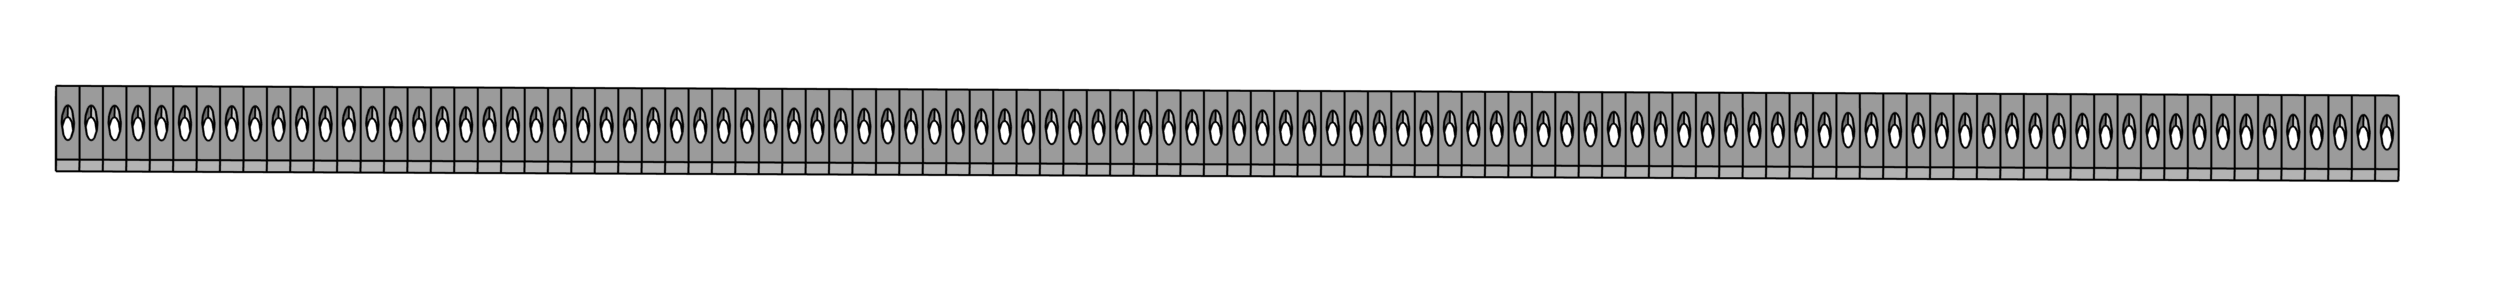
\includegraphics[width=\textwidth]{chapters/results/long_waveguide_geom.png}
	% 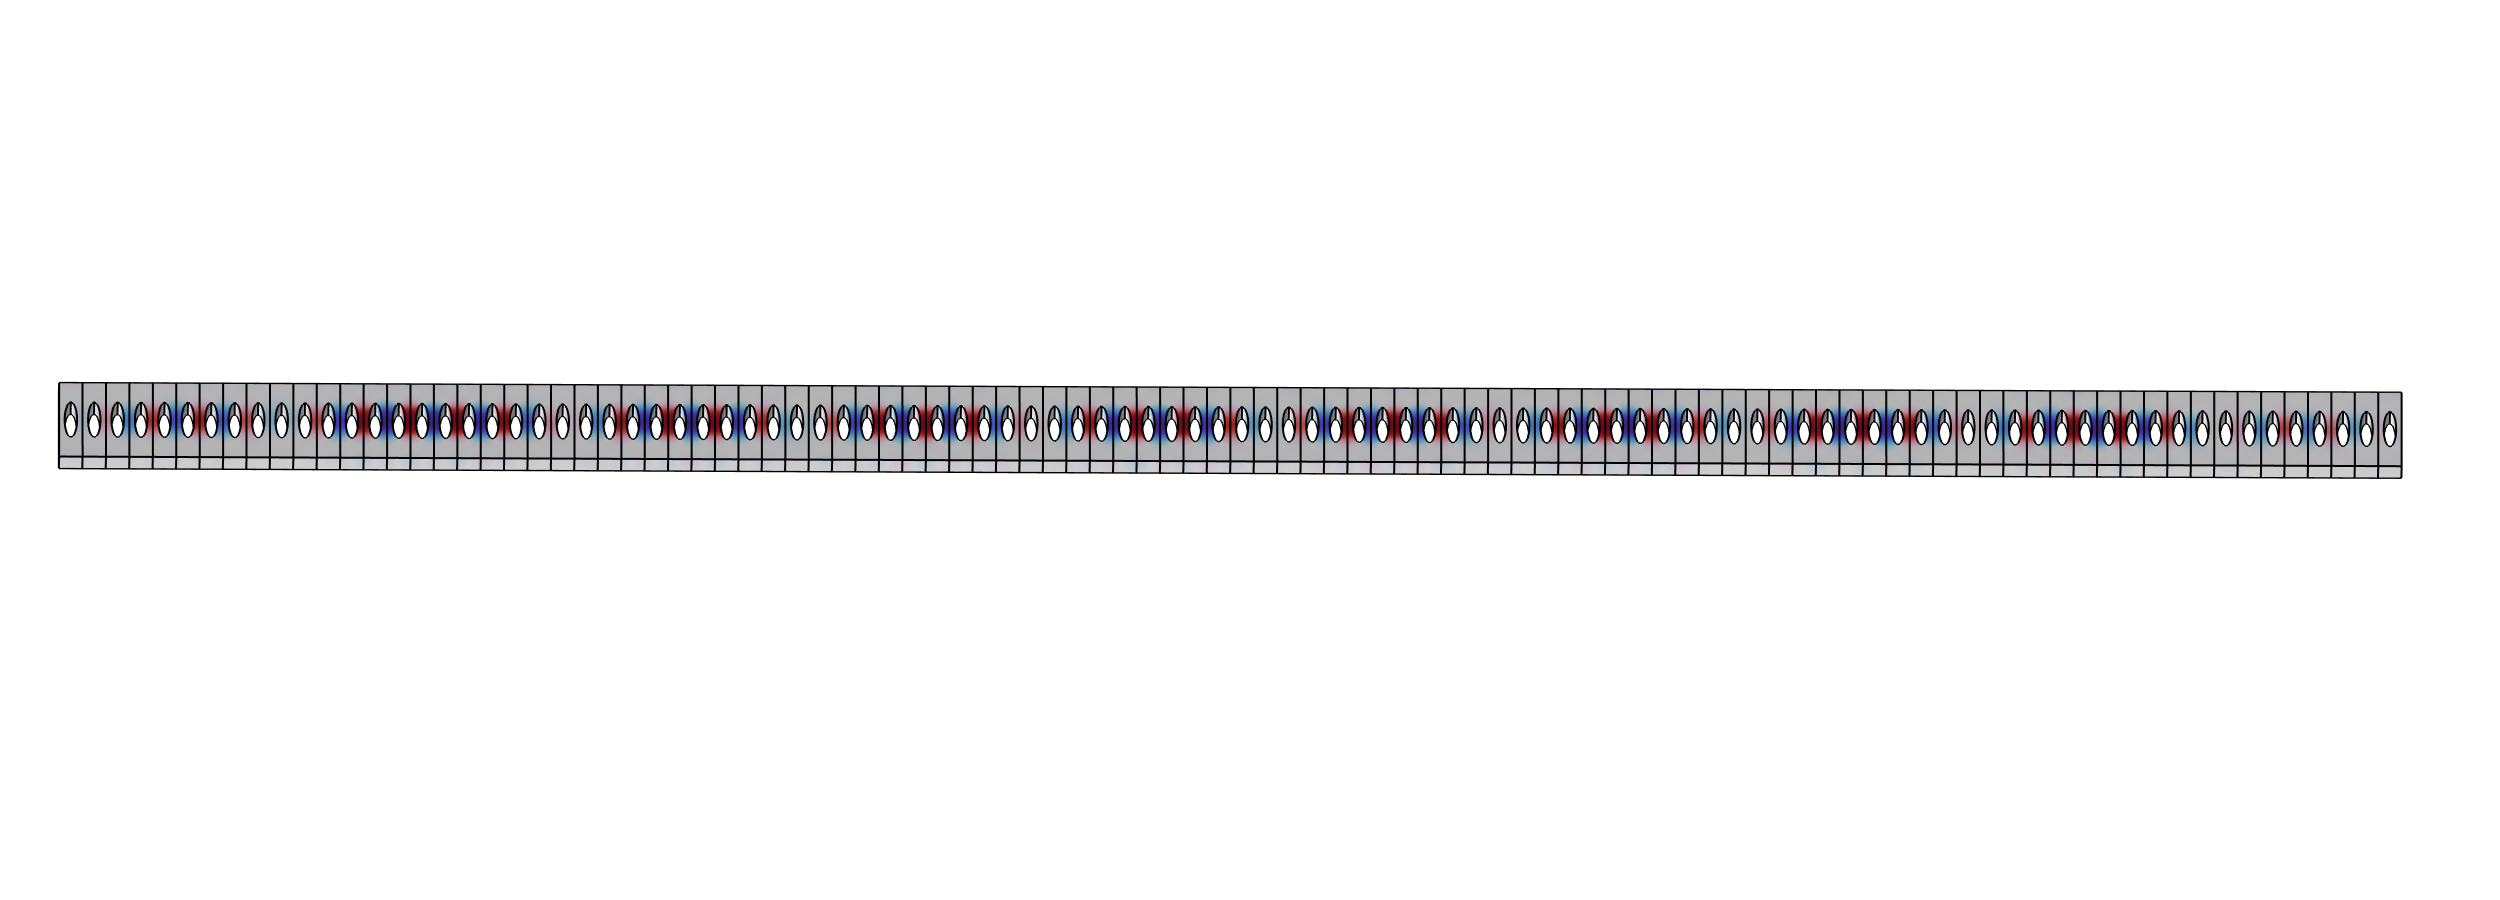
\includegraphics[width=\textwidth]{chapters/results/long_waveguide_v_d=5_s=0.02.png}
	% 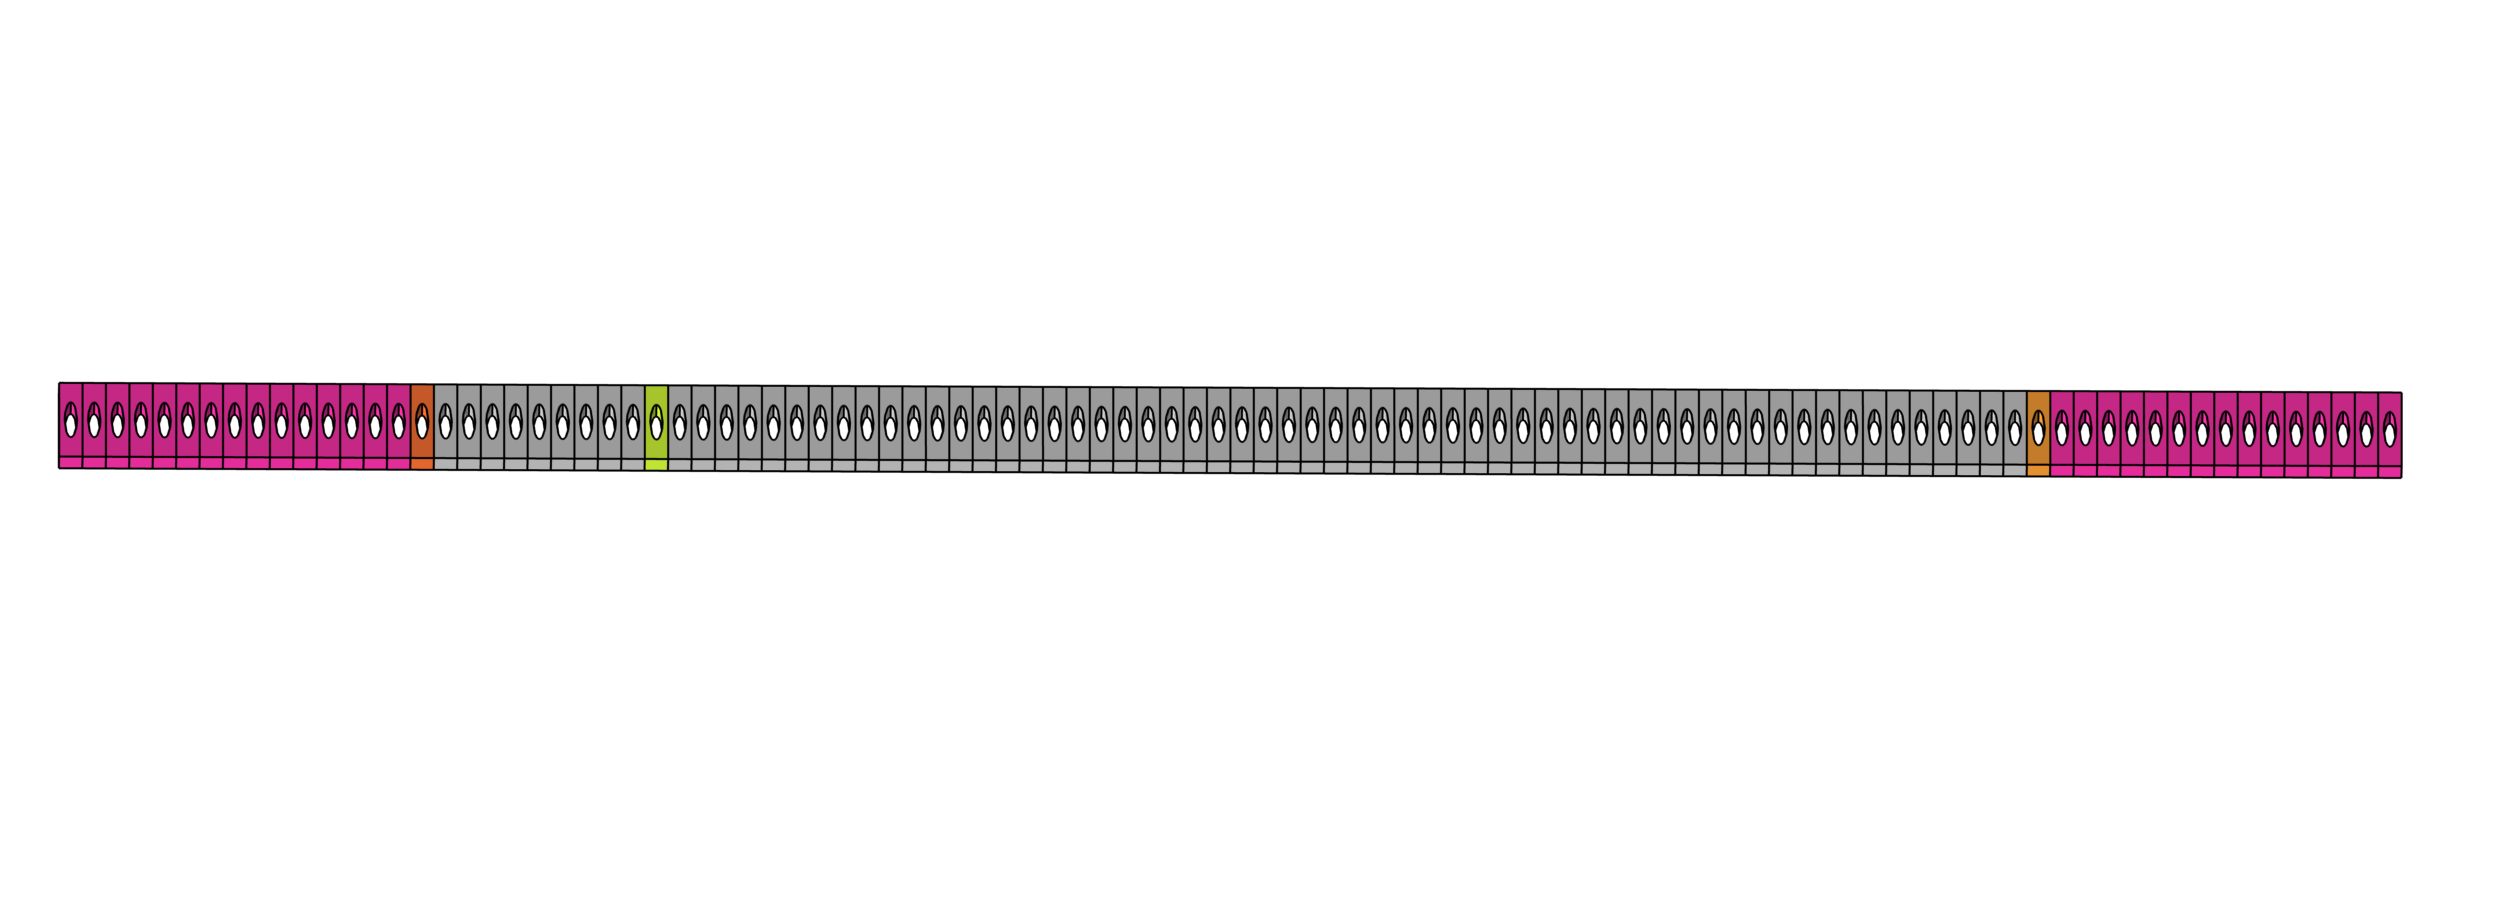
\includegraphics[width=\textwidth]{chapters/results/long_waveguide_selections.png}
	\caption{Thelonwaveide}
	\label{fig:long_waveguide}
\end{figure}

\subsection{PML investigation}

\Cref{fig:pml_sweep1} shows the amplitude of the reflection,
quantified as the peak height relative to the forward propagating wave,
for different profiles.
These figures fit well with the three types of reflection mentioned previously.
To achieve a short yet functional \gls{pml}, $d=5$, $s=0.03$ and $n=20$ was
chosen.

\begin{figure}[htpb]
	\centering
	\begin{subfigure}[]{\textwidth}
	\begin{center}
		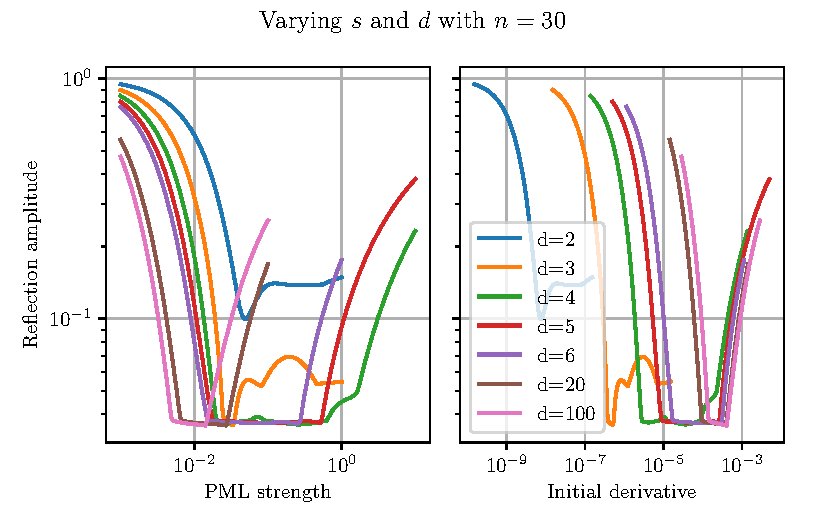
\includegraphics{chapters/methods/pml_sweep_sd.pdf}
	\end{center}
	\caption{
		On the left is the reflection amplitude plotted as a function of the
		\gls{pml} strength $s$ for different $d$.
		For $d > 4$ there are two sources of reflection:
		for small $s$ reflection at the end of the \gls{pml} occurs,
		and for large $s$, there is reflection at the beginning.
		The right figure makes it clear that it is the slope at the beginning of
		the \gls{pml} that matters, since the point at which it becomes
		significant is the same for all $d$.
	}
	\label{fig:pml_sweep_sd}
	\end{subfigure}
	\begin{subfigure}[]{\textwidth}
	\begin{center}
		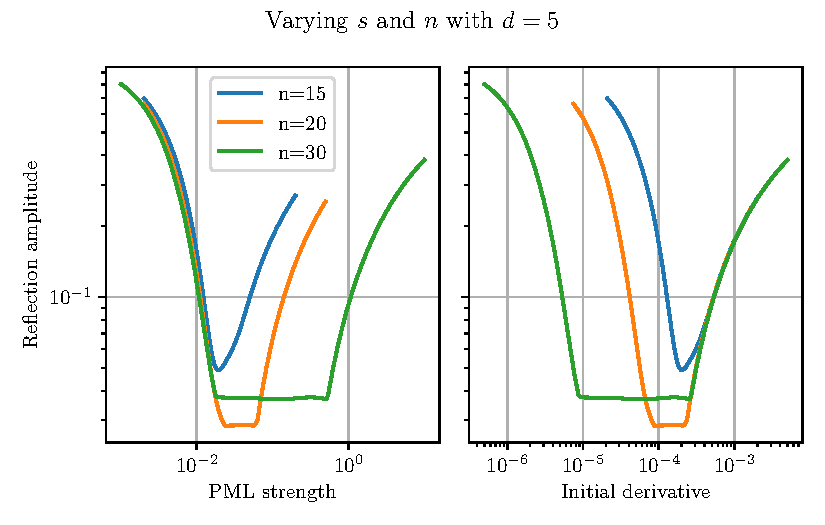
\includegraphics{chapters/methods/pml_sweep_sn.pdf}
	\end{center}
	\caption{
		This is the same as \cref{fig:pml_sweep_sd} but with varying $n$.
		For $n=15$, the reflections from the beginning do not subside before the
		reflections from the end become significant, so at least $n=20$ is
		necessary.
	}
	\label{fig:pml_sweep_sn}
	\end{subfigure}
	\caption{}
	\label{fig:pml_sweep1}
\end{figure}

\subsection{Excitation}

The fact that the excitation was almost solely in the desired mode was verified
in two ways.
Firstly, as detailed in \cref{sec:excitation_method}, $a$ and $b$ in $u = a u_m
+ b u_r$ was computed.
The result was that $a = 1.166$ and $b = 0.0327$.
Thus $99.92\%$ of the energy was in the desired mode.
Secondly, a fourier transform of the y-component of the displacement field was
made.
This can be seen in \cref{fig:v_ft}.
The other modes that could be excited at this frequency have very different wave
vectors, which means that they would show up as separate peaks somewhere around
$0.4 \pi / a$ and $0.1 \pi / a$.
Since no other peaks can be seen, this further supports the result that only the
desired mode is excited.

\begin{figure}[htpb]
	\centering
	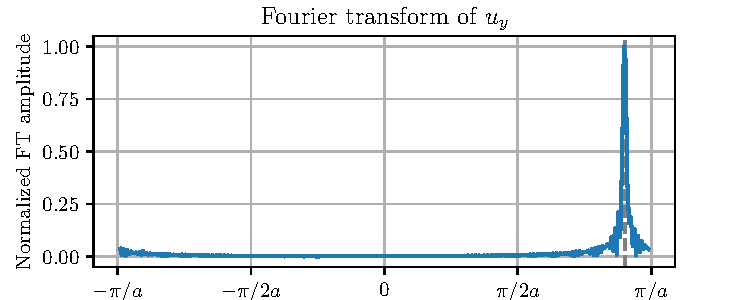
\includegraphics{chapters/results/ft_figure.pdf}
	\caption{%
		Fourier transform of the y-component of the displacement field.
		It clearly shows one wave traveling forward with a k-vector of
		$0.9 \pi / a$, where the dashed gray line is.
		Since the closest other mode at this frequency is at
		$k_y \approx 0.4 \pi / a$, where no peak is visible, it is concluded
		that solely the desired mode is excited.
	}%
	\label{fig:v_ft}
\end{figure}

\section{Continuous optimization}\label{sec:res_cont}

There was a lot of problems with the optimization of the continuous design.
Many optimization runs would end up looking like \cref{fig:bad_cont_conv}.
After switching to the comsol function \mintinline{c}+fsens+ for computing
the derivative, convergence was obtained.
\Cref{fig:cont_conv1} shows the evolution of the transmitted power in one of the
output arms.
This has been normalized such that 1 is the power in through the input waveguide.
Thus, an optimal beamsplitter would reach 0.5.
The figure also shows the power that is reflected back into the input waveguide.
If the powers do not add up, it is because energy is flowing out in a different
mode.
\Cref{fig:cont_design1} shows the design field at the end of the optimization.

\begin{figure}[htpb]
	\centering
	%\includegraphics{}
	\missingfigure{bad convergence plot}
	\caption{}
	\label{fig:bad_cont_conv}
\end{figure}

\begin{figure}[htpb]
	\centering
	\missingfigure{Optimal design}
	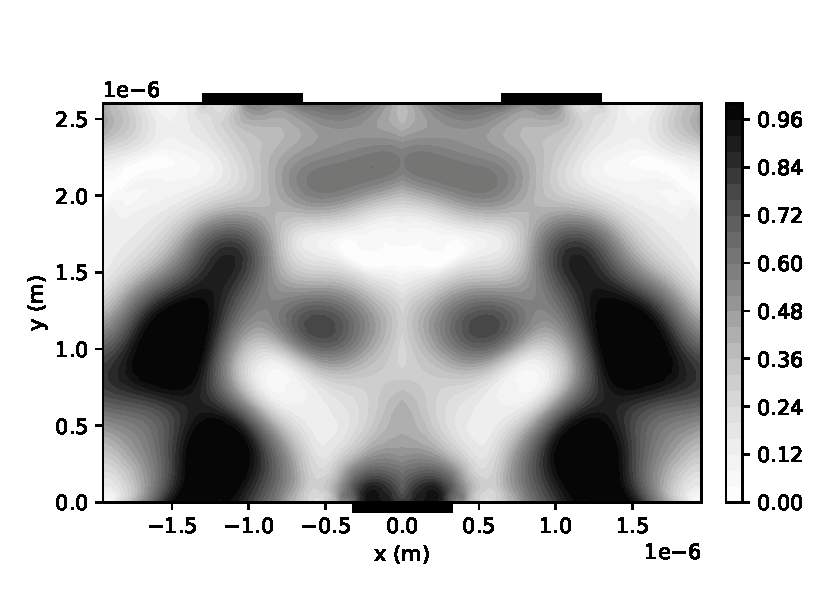
\includegraphics{chapters/results/cont_design1.pdf}
	\caption{This figure shows the }
	\label{fig:cont_design1}
\end{figure}

\begin{figure}[htpb]
	\centering
	%\includegraphics{}
	\missingfigure{Convergence plot}
	\caption{}
	\label{fig:cont_conv1}
\end{figure}

\section{Level-set optimization}\label{sec:res_bin}

Because the continuous optimization didn't converge until rather late,
I could not use the final field of the continuous optimization to initialize the
level-set optimization.
Instead, I tried getting the initial value from a point of the continuous
iteration before it started getting worse again.
I also tried optimizing from a manually drawn guess for the device.

\begin{figure}[htpb]
	\centering
	%\includegraphics{}
	\missingfigure{Optimal design}
	\caption{}
	\label{fig:optimal_bin_design}
\end{figure}

\begin{figure}[htpb]
	\centering
	%\includegraphics{}
	\missingfigure{Convergence plot}
	\caption{}
	\label{fig:convergence_plot_bin}
\end{figure}
